% =====================================================================
\section{The Controller of the Base Paper, in Code}
\label{sec:controller}
% =====================================================================

This section connects each equation of the paper to the lines of \code{paper\_reproduction.py} that implement it. The
derivations and the hand-checkable examples are in the Mathematical Models document; here we only state the
equations again so that the code can be read next to them.

\begin{figure}[H]
\centering
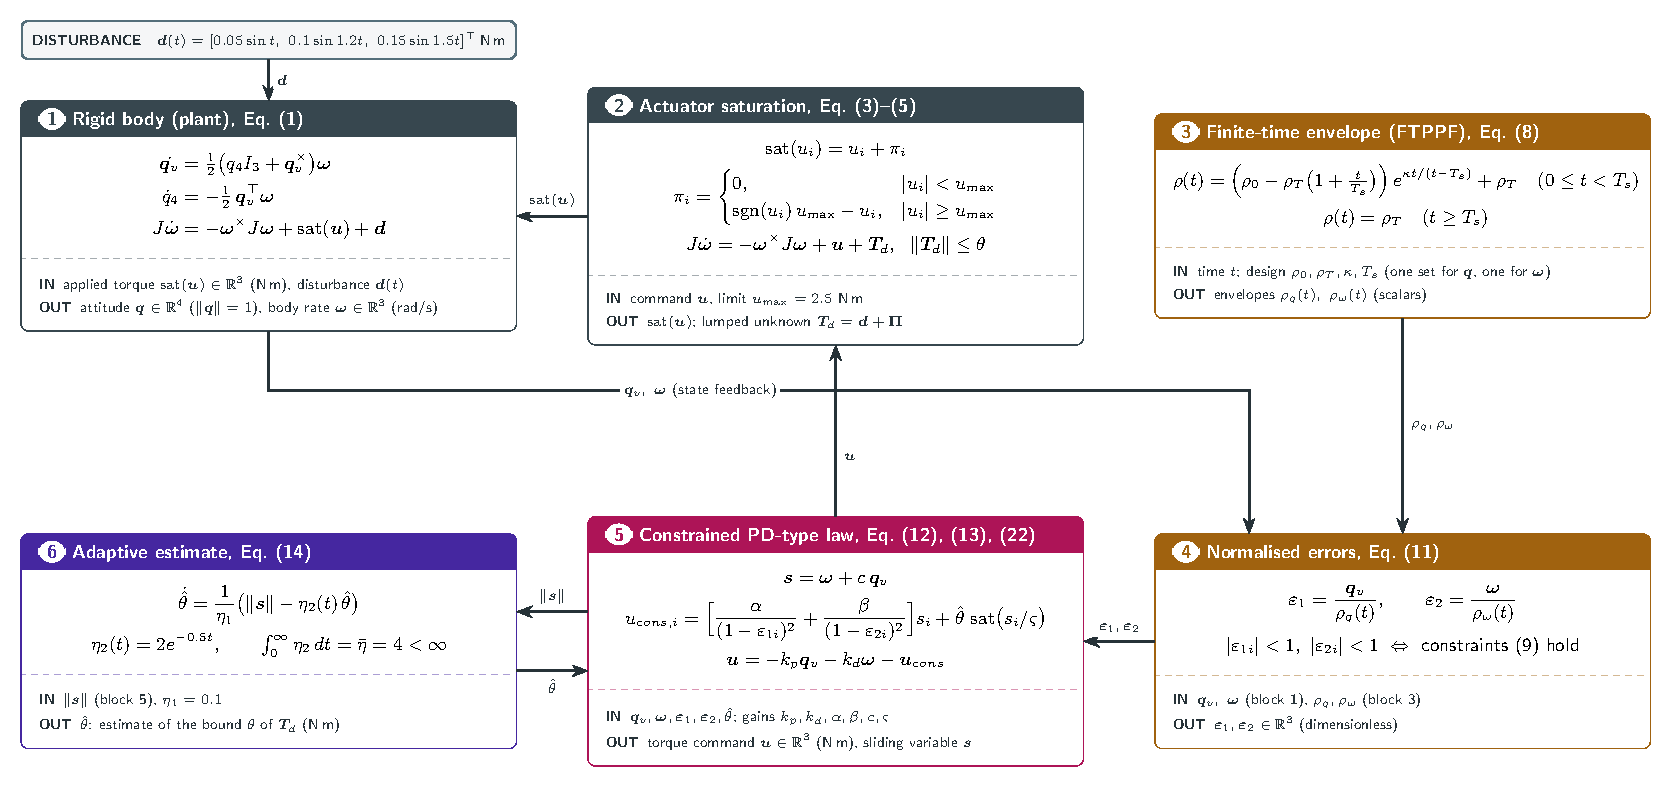
\includegraphics[width=\linewidth]{flow_paper.pdf}
\caption{Equation flow of the paper. Block numbers are used throughout this document.}
\label{fig:flowpaper}
\end{figure}

\subsection{Plant and saturation (blocks 1--2)}

\begin{eqbox}{cPlant}{Eq. (1), (3)--(5)}
\begin{gather*}
\dot\qv=\tfrac12(q_4I_3+\qv^\times)\vw,\qquad \dot q_4=-\tfrac12\qv^\top\vw,\qquad J\dot\vw=-\vw^\times J\vw+\sat(\vu)+\vd\\
\sat(u_i)=\sgn(u_i)\min(|u_i|,\umax)
\end{gather*}
\end{eqbox}
The simulator is written for a whole \emph{batch} of rigid bodies at once (rows of the arrays), which is what makes a
300-run Monte-Carlo study take seconds instead of hours.
\pyfile{107}{114}{\repro}{paper\_reproduction.py --- rhs(): Eq. (1) for a batch}

\subsection{Envelope (block 3)}

\begin{eqbox}{cEnv}{Eq. (8)}
\[
\rho(t)=\Big(\rho_0-\rho_T\big(1+\tfrac{t}{T_s}\big)\Big)\exp\Big(\frac{\kappa t}{t-T_s}\Big)+\rho_T\ \ (0\le t<T_s),\qquad \rho(t)=\rho_T\ \ (t\ge T_s)
\]
\end{eqbox}
\pyfile{78}{85}{\repro}{paper\_reproduction.py --- ftppf(): Eq. (8)}

\resfig{fig01_ppf_comparison.png}{0.8\linewidth}{The finite-time property (cf.\ paper Fig.~2): the FTPPF reaches
$\rho_T$ exactly at $T_s=8$\,s and stays there; the exponential PPF is still $1.67\,\rho_T$ at that time.}{fig:ppf}

\subsection{Normalised errors, control law and adaptation (blocks 4--6)}

\begin{eqbox}{cCtrl}{Eq. (11), (12), (22), (14)}
\begin{gather*}
\veps_1=\frac{\qv}{\rho_q},\qquad \veps_2=\frac{\vw}{\rho_\omega},\qquad \vs=\vw+c\qv,\qquad
\dot\that=\frac{\|\vs\|-\eta_2\that}{\eta_1}\\
u_i=-k_pq_i-k_d\omega_i-\Big(\Big[\frac{\alpha}{(1-\varepsilon_{1i})^2}+\frac{\beta}{(1-\varepsilon_{2i})^2}\Big]s_i+\that\sat(s_i/\varsigma)\Big)
\end{gather*}
\end{eqbox}
\pyfile{117}{140}{\repro}{paper\_reproduction.py --- control(): Eq. (11), (12), (22) and the two comparison controllers}

\subsection{One simulation step}

Per step of 1\,ms: compute the control from the current state, saturate it, update all metrics, integrate the plant
with RK4 holding the torque constant, re-normalise the quaternion, update $\that$.
\pyfile{160}{192}{\repro}{paper\_reproduction.py --- simulate(): the main loop}

\subsection{The barrier form: paper versus symmetric}
\label{sec:barrierform}

\begin{idea}[One-sided or two-sided?]
The paper writes the barrier as $\alpha(1-\varepsilon_{1i})^{-2}$. Read literally, this gain explodes when
$\varepsilon_{1i}\to+1$ but tends to $\alpha/4$ when $\varepsilon_{1i}\to-1$: it guards the upper wall of the tube far more
than the lower wall. The two-sided version $\alpha(1-\varepsilon_{1i}^2)^{-2}$ treats both walls alike. Our first browser
and Gazebo code used the two-sided version without saying so. We now treat the paper form as the reference and report
the symmetric form as a named variant in every table.
\end{idea}

\resfig{fig09_barrier_forms.png}{0.7\linewidth}{Barrier gain as a function of $\varepsilon$ for $\alpha=1.5$.}{fig:barrier}

\begin{toybox}[the same state, two forms]
Part-1 state at $t=0$, axis 3: $\varepsilon_{13}=-0.833$ (closest to its wall of the three axes). Paper form:
$1.5/(1+0.833)^2=0.446$, plus the rate part, $g_3=1.59$. Symmetric form: $1.5/(1-0.694)^2=16.0$, $g_3=17.3$. The paper form
gives the axis that is closest to the wall the \emph{smallest} gain. (MATLAB: \code{step2\_normalised\_error.m}.)
\end{toybox}
